\chapter{Blockchain\label{sec:Blockchain}}

\section{What is Blockchain}
Blockchain advancements isn't simply just single one strategy, however contains Cryptography, science, Algorithm and financial model, consolidating shared systems and utilizing circulated agreement calculation to take care of conventional appropriated database synchronize issue. \\
"Blockchain is a shared innovation, rundown of developing information put away on a conveyed record."
The figure below (see \figref{istw}) shows an example of Blockchian.
\begin{figure}[h]
	\centering
	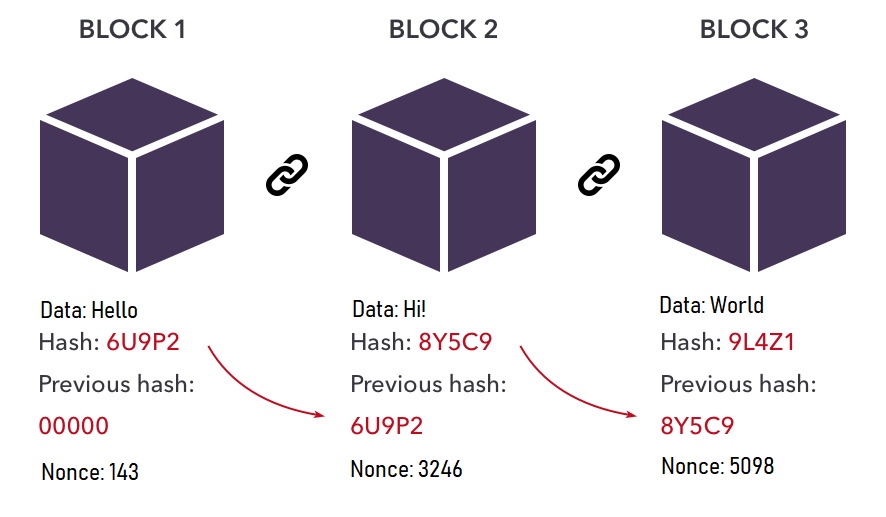
\includegraphics[scale=0.40]{figures/03.png}
	\caption{Blockchain }
	\label{fig:istw}
\end{figure}

\section{Why Blockchain}
\textbf{ De-centralised  }-Information is put away on each and every friend and nobody can adjust it. The hash of your information is created to make variability incomprehensible. Which means an advanced unique mark of your information is made. The blockchain organize is on a very basic level strong and has no-single defenselessness for programmers to abuse.\\
\textbf{ Distributed Ledger  } –Each hub (organization board) approaches the information. We will choose peers who will acknowledge or dismiss at whatever point an exchange occurred (activity made on the blockchain arrange). Means they need to achieve an agreement.\\
\textbf{ Secure  } – The information is put away after some calculation is performed on it. Hashes are created. Means permanence. Put away on various companions never alterable. \\ 
\textbf{ Transparent  } - The information's record by blockchain framework is straightforward to every hub, it additionally straightforward on refresh the information, which is the reason blockchain can be trusted.\\ 

\subsection{Hyperledger }
Their attention is on building up a measured structural system for big business class conveyed records. This incorporates distinguishing normal and basic parts, giving a practical deterioration of a venture blockchain stack into segment layers and modules, institutionalizing interfaces between the segments, and guaranteeing interoperability between records.

\subsection{Introduction Business Blockchain} 
Prerequisites shift. Adaptability, classification, consistence, work process unpredictability, and even security necessities contrast definitely crosswise over businesses and employments. Every one of these prerequisites, and numerous others, speak to a conceivably remarkable advancement point for the innovation. \\
The Hyperledger Architecture has recognized the accompanying business blockchain parts:\\
\textbf{ Consensus Layer   }-In charge of producing a concession to the request and affirming the accuracy of the arrangement of exchanges that comprise a square.\\
\textbf{ Smart Contract Layer   }-In charge of preparing exchange asks for and deciding whether exchanges are legitimate by executing business rationale.\\
\textbf{ Communication Layer   }-In charge of preparing exchange asks for and deciding whether exchanges are legitimate by executing business rationale.\\
\textbf{ Data Store Abstraction   }-Permits distinctive information stores to be utilized by different modules.\\
\textbf{ Crypto Abstraction    }-Permits diverse crypto calculations or modules to be swapped out without influencing different modules.\\
\textbf{ Identity Services   }-Empowers the foundation of a base of trust amid set-up of a blockchain occasion, the enlistment and enrollment of characters or framework elements amid system task, and the administration of changes like drops, includes, and renouncement. Additionally, gives verification and approval.The figure below (see \figref{iste}) shows.\\
\begin{figure}[h]
	\centering
	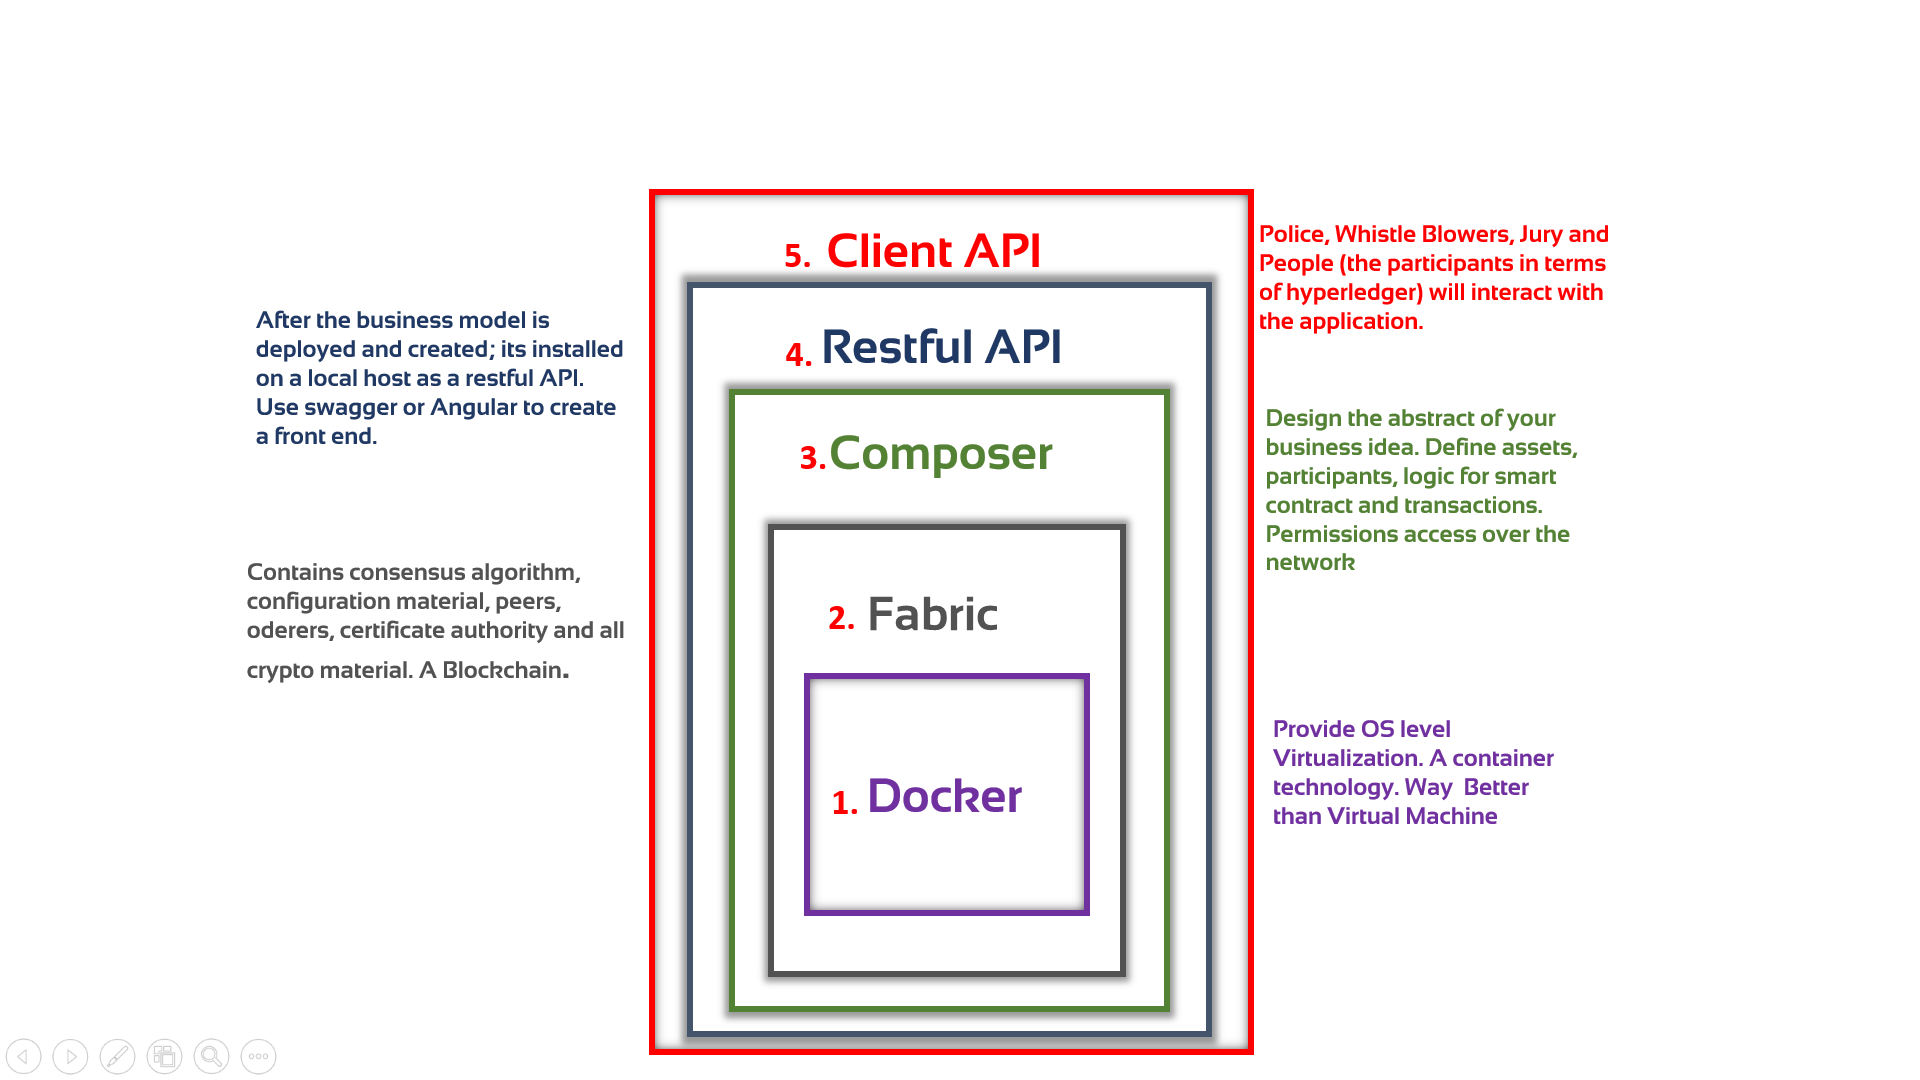
\includegraphics[scale=0.40]{figures/04.png}
	\caption{Blockchain }
	\label{fig:iste}
\end{figure}

\subsection{Hyperledger Fabric }
An open source undertaking grade per-mission circulated record innovation (DLT) stage, intended for use in big business settings, which conveys some key separating abilities over other famous appropriated record or blockchain stages. One key purpose of separation is that Hyperledger was set up under the Linux Foundation, which itself has a long and exceptionally effective history of supporting open source extends under open administration that become solid continuing networks and flourishing eco frameworks. \\
Hyperledger is administered by adverse specialized controlling advisory group, and the Hyperledger Fabric venture by a various arrangement of maintainers from numerous associations.\\ 
Texture is involved the accompanying measured parts:
\begin{itemize}
	\item A pluggable requesting administration builds up agreement on the request of exchanges and afterward communicates squares to peers.
	\item  A pluggable enrolment specialist co-op is in charge of partner elements in the system with cryptographic personalities.
	\item  A discretionary distributed babble benefit disperses the squares yield by requesting administration to different friends.
	\item  Savvy contracts ("chaincode") keep running inside a compartment domain (e.g. Docker) for separation. They can be written in standard programming dialects however don't have guide access to the record state.
	
\end{itemize}
\section{Hyperledger and Our Application }
\subsection{Hyperledger Composer}
It resembles a complier of Hyperledger Fabric. In arranger, we need to characterize our business organize. The exchanges and chain codes working. We here characterize our business organize rationale and test it on arranger play area before going ahead. \\
The fundamental parts of our Hyperledger Composer are.\\
\textbf{ Participants  }-One’s who is going to interact with the system. The Police, Whistle-Blower and the Jury.\\
\textbf{ 	Assets   }-Evidence and Cases. Any commodity which can be sold to the subscriber is an asset.\\
\textbf{ 	Transaction   }-The logic of chaincode responsible for validation and verification of every action happening on our blockchain.\\  
\textbf{ Query  }-To apply filters. Search specifically under given rates.\\
\textbf{ 	Permissions   }- An acl file to control read and write operation of participants over the network.
Combine together they make a .bna file which is later installed on a blockchain cloud.The figure below (see \figref{istg}) shows Hyperledger Architecture.\\
\begin{figure}[h]
	\centering
	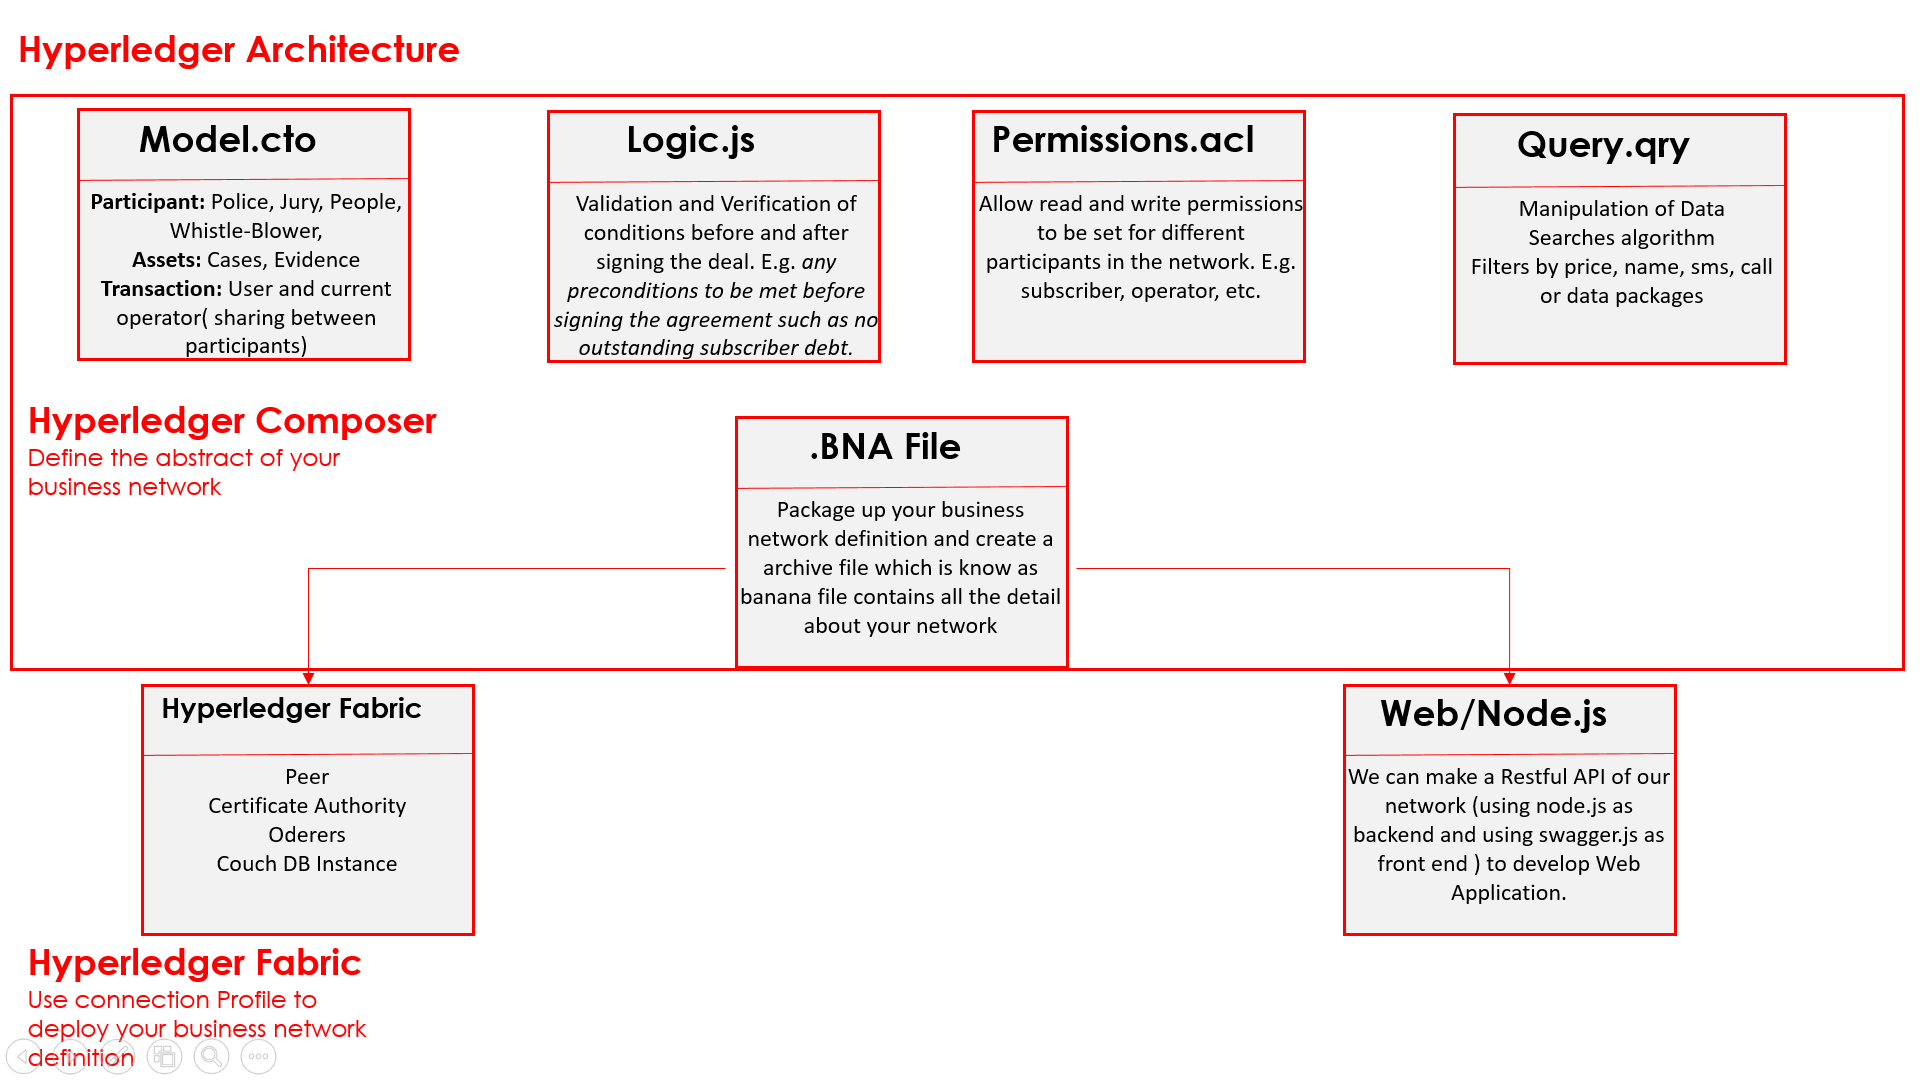
\includegraphics[scale=0.40]{figures/05.png}
	\caption{Hyperledger Composer }
	\label{fig:istg}
\end{figure}
\subsection{IBM Cloud }
Cloud means a hosting service. Since it is not same as we host a simple website so we refer it as a blockchain cloud. The two main and famous clouds for hosting Hyperledger Blockchain Network are:

\begin{itemize}
	\item Amazon Web Services
	\item IBM Blockchain Cloud
	
\end{itemize}
These two platforms officially gives you an instance of Hyperledger Fabric which will interact with our .bna file.
Except that on every single Cloud Platform we have to manually install Hyperledger Fabric and Composer. Which will cost space and increase a lot of workload. We were testing IBM 
\subsection{Hyperledger Fabric}
Once the .bna file is created it has to interact with the Fabric.\\
Three main components of Hyperledger Fabric are: \\
\textbf{ Peer  }-The administrators are our friends which will embrace and perform agreement on arrangements.\\
\textbf{ Oderers  }-At whatever point a demand originate from endorser, to make it reach to companions and include it into blockchain arrange is its duty. Synchronization of correspondence on blockchain.\\
\textbf{Certificate Authority }-Gives administrator access to include peers create ssl endorsement and private and open keys for friends to maintain a strategic distance from breakdown and make netwoek secure. \\
As should be obvious in the image above once the IBM Blockchain Cloud account is made it straightforwardly gives you access to IBM Hyperledger Fabric Instance as every one of the three segments of Hyperledger Fabric are running, we simply need to introduce our .bna record in introduce code area.\\
\textbf{Channels }-We can make distinctive diverts in one blockchain arrange. We can likewise include diverse companions in that channel. One application is for one occasion inside that there are distinctive channels. 
Channels are utilized to have private correspondence.\\
For example you have private members you can add special peers and create separate chain for them.